\documentclass[12pt,a4paper]{article}

\usepackage[utf8]{inputenc}
\usepackage[portuguese,brazil,english]{babel}
\usepackage[a4paper, inner=3cm, top=3cm, outer=2cm, bottom=2cm]{geometry}
\usepackage[onehalfspacing]{setspace}
\usepackage{xspace}
\usepackage{fancyhdr}
\usepackage[dvips]{graphicx}
\usepackage{blindtext}
\usepackage{caption}
\usepackage{multirow}

\DeclareGraphicsExtensions{.eps}

\def\registered{\textsuperscript{\textregistered}}
\def\trademark{\textsuperscript{\texttrademark}}
\def\Intel{Intel\registered\xspace}
\def\AMD{AMD\registered\xspace}
\def\IBM{IBM\registered\xspace}
\def\SunMicro{Sun~Microsystems\registered\xspace}
\def\Oracle{Oracle\registered\xspace}
\def\Sun{Sun\registered\xspace}
\def\SystemZ{{\it System~Z}\trademark\xspace}
\def\zEC{{\it zEC12}\trademark\xspace}
\def\zEnt{{\it zEnterprise}\trademark\xspace}
\def\mainframe{{\it mainframe}\xspace}
\def\mainframes{{\it mainframes}\xspace}
\def\BlueGeneQ{{\it Blue~Gene/Q}\trademark\xspace}
\def\Rock{{\it Rock}\trademark\xspace}
\def\ASF{{\it ASF}\trademark\xspace}
\def\ASFlong{{\it Advanced Synchronization Facility}}
\def\SandyBridge{{\it Sandy~Bridge}\trademark\xspace}
\def\Haswell{{\it Haswell}\trademark\xspace}
\def\STAMP{{\it Stanford Transactional Applications for Multi-Processing}}
\def\ILP{{\it Instruction Level Parallelism}}
\def\multicore{{\it multicore}\xspace}
\def\core{{\it core}\xspace}
\def\cores{{\it cores}\xspace}
\def\thread{{\it thread}\xspace}
\def\threads{{\it threads}\xspace}
\def\ACID{{\it Atomicity, Consistency, Isolation and Durability}}
\def\checkpoint{{\it checkpoint}\xspace}
\def\commit{{\it commit}\xspace}
\def\eager{{\it eager}\xspace}
\def\lazy{{\it lazy}\xspace}
\def\buffer{{\it buffer}\xspace}
\def\buffers{{\it buffers}\xspace}
\def\overflow{{\it overflow}\xspace}
\def\rollback{{\it rollback}\xspace}
\def\fallback{{\it fallback}\xspace}
\def\abort{{\it abort}\xspace}
\def\aborts{{\it aborts}\xspace}
\def\hardware{{\it hardware}\xspace}
\def\software{{\it software}\xspace}
\def\store{{\it store}\xspace}
\def\SMT{{\it Simultaneous Multi-Threaded Threads}}
\def\TSX{{\it Transactional Synchronization Extension}}
\def\RTM{{\it Restricted Transactional Memory}}
\def\HLE{{\it Hardware Lock Elision}}
\def\TLB{{\it Translation Look-Aside Buffer}\xspace}
\def\lock{{\it lock}\xspace}
\def\unlock{{\it unlock}\xspace}
\def\xbegin{{\tt xbegin}\xspace}
\def\xabort{{\tt xabort}\xspace}
\def\xend{{\tt xend}\xspace}
\def\PCM{{\it Performance Counters Monitor}}
\def\lock{{\it lock}\xspace}
\def\locks{{\it locks}\xspace}

\begin{document}

\pagestyle{fancy}
\fancyhf{} % clear head and foot fields
% page number (\thepage) at center [C] in boldface
%\fancyfoot[C]{\thepage}
% override default head rule thickness
\renewcommand{\headrulewidth}{0.8pt}
% override default sectionmark -- simple section name (\thesection) and number {#1} in boldface
\renewcommand{\sectionmark}[1]{\markright{\bfseries \thesection\ #1}}
% override default subsectionmark -- simple section name (\thesubsection) and number {#1} in boldface
\renewcommand{\subsectionmark}[1]{\markright{\bfseries \thesubsection\ #1}}
% defines what to show on the right part of the header
\fancyhead[LH]{\nouppercase{\rightmark}}
\fancyhead[RH]{{\bfseries \thepage}}
\selectlanguage{portuguese}

%-------------------------------
% CAPA
%-------------------------------
\thispagestyle{empty}
\begin{titlepage}

	\begin{center}
		 {\large \textbf{\textsf{Universidade Estadual Paulista}}}\\
		 {\large \textbf{\textsf{Instituto de Geociências e Ciências Exatas}}}\\
		 {\large \textbf{\textsf{Campos de Rio Claro}}}

		\vspace{4cm}

		{\Large \textsf{Lucas Bagatini do Nascimento}}

		\vspace{4cm}

		%\rule{\linewidth}{1mm}\vspace{4mm}
		{\LARGE \textbf{\textsf{TODO: título?}}}
		%\rule{\linewidth}{1mm}

		\vfill

		Rio Claro -- SP,\\
		\the\year
	\end{center}


\end{titlepage}

%-------------------------------
% FOLHA DE ROSTO
%-------------------------------
\thispagestyle{empty}
\begin{titlepage}
	\begin{center}
		{\large \textsf{Lucas Bagatini do Nascimento}}

		\vspace{3cm}

		%\rule{\linewidth}{1mm}\vspace{4mm}
		{\LARGE \textbf{\textsf{TODO: título?}}}
		%\rule{\linewidth}{1mm}
	\end{center}

	\vspace{3cm}

	\hfill
		\begin{minipage}[c]{0.6\columnwidth}
			Trabalho de Conclusão do Curso, modalidade Trabalho de Graduação, apresentado
			no 1º semestre letivo de \the\year,  à disciplina ES/TG do Curso de Bacharelado em Ciências
			da Computação, período Integral, do Instituto de Geociências e Ciências Exatas
			da Universidade Estadual Paulista “Júlio de Mesquita Filho”, campus de Rio Claro,
			para apreciação segundo as normas estabelecidas pelo Conselho do Curso, em 02/09/2021.\\

			\textbf{Orientador:~}\textsf{Prof.~Dr.~Alexandro José Baldassin} \\
			\textbf{Departamento:~}\textsf{Dept.~de Estatística, Matemática Aplicada e Computação (DEMAC)}
		\end{minipage}

	\vfill

	\begin{center}
		Rio Claro -- SP,\\
		\the\year
	\end{center}

\end{titlepage}

%-------------------------------
% FOLHA DE APROVAÇÃO
%-------------------------------
%\thispagestyle{empty}
%\begin{titlepage}
%	\begin{center}
%		{\large \textsf{Lucas Bagatini do Nascimento}}
%
%		\vspace{2cm}
%
%		{\large \textbf{\textsf{TODO: título?}}}
%	\end{center}
%
%	\vspace{7cm}
%
%	\begin{center}
%		{\large Comissão Examinadora} \\[6.5mm]
%
%		\underline{\hspace{10cm}} \\
%		Prof.~Dr.~Alexandro José Baldassin -- Orientador\\
%		Departamento de Estatística, Matemática Aplicada e Computação\\
%		Universidade Estadual Paulista -- UNESP\\[6.5mm]
%
%		\underline{\hspace{10cm}} \\
%		Prof.~Dr.~TODO:preencher nome da banca\\
%		Departamento de Estatística, Matemática Aplicada e Computação\\
%		Universidade Estadual Paulista -- UNESP\\[6.5mm]
%
%		\underline{\hspace{10cm}} \\
%		Prof.~Dr.~TODO:preencher nome da banca\\
%		Departamento de Estatística, Matemática Aplicada e Computação\\
%		Universidade Estadual Paulista -- UNESP
%	\end{center}
%
%	\vfill
%
%	\begin{center}
%		Rio Claro -- SP, \underline{\hspace{1cm}} de \underline{\hspace{3cm}} de \the\year
%	\end{center}
%
%\end{titlepage}

%-------------------------------
% RESUMO EM PORTUGUÊS
%-------------------------------
\thispagestyle{empty}
\begin{center}
\section*{RESUMO}
\end{center}

TODO: fazer resumooooo ç__ç

\newpage

%-------------------------------
% RESUMO EM INGLÊS
%-------------------------------
\thispagestyle{empty}
\begin{center}
\section*{ABSTRACT}
\end{center}

TODO: do the abstraaaaact ç__ç

\newpage

%-------------------------------
% SUMÁRIO
%-------------------------------
\thispagestyle{empty}
\renewcommand*\contentsname{SUMÁRIO}
\begin{center}
\tableofcontents
\end{center}
\newpage

%-------------------------------
% INTRODUÇÃO
%-------------------------------
\section{Introdução}

Motivado pela iminente desaceleração (e possível fim) da anciã Lei de Moore, neste trabalho, pretende-se fazer uma comparação quantitativa, mas principalmente qualitativa, entre as abordagens de 4 linguagens modernas de programação ao paralelismo e concorrência. As linguagens foram escolhidas por sua diversidade, relevância, propósito e ferramentas implementadas e embutidas em seu \emph{design}: Python (utilizando \emph{thread pooling} e \emph{process pooling}), Rust, Go e Kotlin.

A Lei de Moore (que surgiu como observação, não como predição), dita que a cada dois anos a densidade de transistores de um processador dobraria~\cite{moore1965cramming}. Aproximando-se dos limites físicos~\cite{seabaugh2013tunneling} do ``aço e silício'', a humanidade revisita velhos métodos de dividir tarefas computacionalmente exigentes, embutindo em linguagemns de programação as novas incarnações de antigas ferramentas como mutexes e troca de mensagens, revigorando o campo de paralelismo e concorrência e soprando novo fôlego às tecnologias atuais de transistores.

O estudo ocorreu em duas etapas: na primeira, dois problemas trivialmente paralelizáveis foram resolvidos utilizando cada uma da linguagens (computação do número pi através da série de Leibniz e a multiplicação de duas matrizes). Com códigos em mãos, foi possível executá-los, tendo como parâmetro a quantidade de threads nas quais seriam executados, e daí, traçar um perfil da eficiência e ganho de desempenho e formular uma comparação quantitativa. Mais importante, contudo, foi a análise qualitativa da usabilidade e facilidade de adoção das linguagens e conceitos que trazem à discussão.

Pretendia-se, adicionalmente, abordar Haskell por ser uma linguagem funcional poderosa com um compilador robusto e intrincado, mas não houve tempo hábil para tal. Teria sido uma inclusão interessante, não somente pela mudança de paradigma, mas pelo fato de haskell possuir dados imutáveis por padrão e aprender essa linguagem quase taumatúrgica seria um experimento interessante. Basta dizer que para os ``não iniciados'', Haskell é no mínimo esotérico e arcano. Também seria uma adição interessante pela comparação de desempenho, já que há o mito de que Haskell não consegue competir com linguagens mais tradicionais, apesar de ser compilado.

As linguagens se provaram competentes no que se propunham: Go é extraordinariamente acessível, Kotlin é tão ubíquto quanto Java, Rust é rápido como relâmpago e Python permanece capaz de tudo um pouco. Das linguagens, Python foi de longe a mais lenta, o que já se esperava. Surpreendentemente, Python não se mostrou a mais conveniente do grupo. Rust permanece desafiador, mas recompensador, enquanto Kotlin se mantém íntimo do mercado, sendo financiada (e influenciada) pela empresa JetBrains.


\newpage
%-------------------------------
% CONTEXTUALIZAÇÃO TEÓRICA
%-------------------------------
\section{Contextualização Teórica}

Neste capítulo serão abordados termos e conceitos centrais ao tema tratado: a diferença entre Paralelismo e Concorrência (Seção~\ref{ssec:concorrencia e paralelismo}), alguns problemas comuns que atormentam programadores que enfrentam algoritmos paralelos (Seção~\ref{ssec:problemas comuns}), algumas ferramentas clássicas utilizadas para sincronizar e paralelizar algoritmos (Seção~\ref{ssec:ferramentas classicas sincronizacao paralelizacao}), alguns dos modelos de paralelismo (Seção~\ref{ssec:modelos paralelismo}) em especial os utilizaos pelas linguagens estudadas: Python, Go, Kotlin e Rust.

\subsection{Motivação: Limites Físicos da Lei de Moore}

É inegável a importância da computação para a civilização humana moderna. É sabido também que a demanda por poder computacional vem crescendo vertiginosamente (em inúmeras áreas, desde a academia ao entretenimento) e até recentemente a microeletrônica foi capaz de acompanhar, reduzindo o tamanho dos componentes (em especial transistores) e produzindo chips cada vez mais complexos e poderosos~\footnote{https://www.phonearena.com/news/A-modern-smartphone-or-a-vintage-supercomputer-which-is-more-powerful\_id57149, acessado em 24/08/2021}. As maiores maravilhas da ciência dos últimos séculos cabem em uma miúda caixa de aço e silício em nossos bolsos, mas a tendência de incrementar mais e mais os processadores e chips está chegando em seu limite, a menos que surjam métodos revolucionários~\cite{powell2008quantum}.

A Lei de Moore, postulada por Gordon E. Moore em 1965 e revisada em 1975~\cite{moore1965cramming}, afirma que a cada dois anos a densidade de transistores dobraria, fazendo crescer consigo a potência dos dispositivos. Não é surpresa que eventualmente um limite superior seria atingido sem uma mudança radical de paradigma. Dentre as razões estão: a imensa complexidade da microeletrônica envolvida, a impossibilidade de se resfriar os componentes, e vazamentos da corrente~\cite{seabaugh2013tunneling}. Ironicamente, o tunelamento de elétrons que outrora destruía os dados em transistores pequenos demais, está sendo estudado como viabilizador de um novo tipo de transistor, batizado Tunnel FET ou TFET~\cite{seabaugh2013tunneling}.

Com tais limitações físicas em mente, abordagens outrora típicas de ficção científica vem sendo estudadas, como super materiais com características estranhas e computação quântica. Contudo, por agora, a melhor solução para a definhante Lei de Moore é adaptar e refinar a tecnologia existente, desenvolvendo as áreas de computação distribuída e computação paralela.

Um novo modo de programar demanda novas ferramentas e traz consigo novos desafios.

\subsection{Concorrência e Paralelismo}
\label{ssec:concorrencia e paralelismo}

Baseado nas definições trazidas por Peter Pacheco~\cite{pacheco11}, podemos definir concorrência como o trabalho sobre múltiplas tarefas por um mesmo agente, alternadamente. Ou seja, certos passos das múltiplas tarefas são intercalados uns com os outros e se faz progresso em todas.

Uma analogia: Um estudante deseja passar em uma disciplina da graduação (cálculo 3) e resolve apelar para a superstição, confeccionando 1000 tsurus (pequenas dobraduras de cegonhas). Se fizesse uma a uma, do começo ao fim, trataria-se de uma abordagem sequencial (ou serial). O estudante decide fazer os tsurus parcialmente e depois retomar e terminar as dobraduras incompletas pois julga que será menos tedioso. Esta é uma abordagem concorrente (um agente alternando entre várias tarefas, iguais neste exemplo).

Paralelismo, por outro lado, demanda simultaneidade dos passos das diversas tarefas por diversos agentes. Os passos não são intercalados e as tarefas são desenvolvidas simultaneamente (mas não necessariamente sincronizadas ou emparelhadas, se forem tarefas iguais).

Retomando a analogia: Os amigos do estudante também estão com dificuldades e resolvem ajudar para receberem boa sorte. Cada um pega um punhado de papéis de dobradura e fazem, ao mesmo tempo, os tsurus. Alguns são mais rápidos e outros demoram mais para aprender, então neste exemplo o desenvolvimento das tarefas acontece em ritmos diferentes.

De acordo com esta definição um sistema que admite paralelismo, como o grupo de alunos como um todo, é necessariamente concorrente, ou seja, mesmo que cada agente que faz parte do grupo desempenhe suas tarefas sequencialmente, o grupo desempenha tarefas concorrentemente. Quando se trata de computadores, costuma-se chamar cada um desses agentes de \textbf{thread}.

\subsection{Speedup e Lei de Amdahl}
\label{ssec:lei de amdahl}

 Praticamente todos os algoritmos possuem seções sequenciais, nem que sejam somente o início e o fim (como os casos estudados nos experimentos, chamados trivialmente paralelizáveis ou embaraçosamente paralelizáveis~\cite{pacheco11}).

Uma seção do algoritmo é dita sequencial se seus passos dependem dos resultados uns dos outros. Na analogia do estudante e seus tsurus: cada uma das dobras deve ser feita em sequência. Não faz sentido detalhar o bico da ave se o pescoço ainda nem foi dobrado.

O fator de redução do tempo gasto para desempenhar uma tarefa através de um novo algoritmo (paralelizando-o, nesse caso) é chamado de speedup. Em um computador ideal, pode-se dizer que o ganho de eficiência é limitado somente pelas seções sequenciais do algoritmo. Na prática isso não ocorre pois a cada nova thread criada há o esforço de gerenciamento de recursos e eventual destruição das threads impossibilitando o comportamento assintótico do speedup quando se aumenta o número de threads. Na analogia do estuadnte e seus tsurus: se conseguisse que o campus todo contribuísse (1000 alunos) e cada um fizesse um único tsuru, a tarefa ainda demoraria o tempo necessário para fazer uma dobradura (seção sequencial). O milésimo-primeiro aluno não seria capaz de acelerar o processo dos outros.

Outro exemplo muito comum e ironizado é a gravidez típica, que necessariamente dura 9 meses. Duas pessoas são incapazes de entregar um bebê em quatro meses e meio.

A Lei de Amdahl~\cite{bryant2003computer} formaliza o speedup máximo obtido em um programa:

\begin{equation}
\label{formula:amdahl}
    S_{latency} \left ( s \right ) = \frac{1}{\left ( 1 - p\right )+ \frac{p}{s}}
\end{equation}

Onde $S_{latency}$ é speedup relativo à latência (ou speedup de tempo de execução) do algoritmo todo; $s$ é o speedup da seção paralelizável; $p$ é a parcela do código que é paralelizável.

Percebe-se que se o speedup $s$ da seção paralelizável tender ao infinito (com infinitas threads, por exemplo), o tempo total de execução do algoritmo tende à soma das seções sequenciais.

Por exemplo: uma tarefa que originalmente levava 20 segundos para ser concluída pode ser paralelizada parcialmente. Sabe-se que $1/2$ dela pode ser paralelizada ($p=1/2$) e o computador místico é capaz de utilizar infinitas threads e dividir o trabalho instantâneamente, levando a um speedup infinito ($s \to \infty$). De acordo com a fórmula \ref{formula:amdahl} da Lei de Amdahl, chega-se à conlcusão de que o speedup máximo é de 2 vezes, ou seja, ao utilizar um computador digno de ficção científica o algoritmo tomará, no mínimo, 10 segundos.

Na prática, o custo combinado do gerenciamento das threads cresce junto com o número de threads, produzindo um ponto de mínimo no qual o ganho é máximo em comparação ao incremento.

\subsection{Problemas Comuns de Algoritmos Paralelos}
\label{ssec:problemas comuns}

A paralelização de algoritmos nem sempre é trivial. Além de certos trechos não serem paralelizáveis, durante a execução não há garantias acerca da ordem de execução dos passos entre threads, ou seja, não há garantias de que uma thread alcança um certo ponto do algoritmo antes da outra, comprometendo a integridade dos resultados. Serão abordados alguns dos problemas mais comuns de algoritmos paralelos a seguir.

\subsubsection{Corrida, Atomicidade e Seções Críticas}
\label{sssec:corrida atomicidade e secoes criticas}

Quando duas threads estão sendo executadas simultaneamente e compartilham uma variável, é possível que ambas tentem acessar o valor ao mesmo tempo (ou uma acesse o valor antes que a outra termine de atualizá-lo). Desse modo, o resultado depende de qual thread acessa a variável primeiro, corrompendo o resultado e tornando-o incerto. Chamamos isso de \textbf{condição de corrida}~\cite{pacheco11}. Quaisquer seções de código suscetíveis a condições de corrida e que demandam que uma única thread acesse um dado recurso são chamadas \textbf{seções críticas}~\cite{pacheco11}.

Pode-se estender a definição de seção crítica para códigos concorrentes mantendo em mente a ideia de atomicidade: se há dependência direta do resultado de uma computação (leitura ou escrita inclusos), então é imperativo que nenhum outro processo, paralelo ou concorrente, utilize os valores atuais antes que tal computação seja concluída, ou seja, a computação deve ser \textbf{atômica}, (já que tentativas de acesso não podem ser simultâneas).

\subsubsection{Atomicidade}
\label{sssec:atomicidade e secoes criticas}

Caso duas ou mais threads compartilhem uma mesma variável, é necessário garantir a atomicidade das operações sobre ela, ou seja, deve-se garantir que o scheduler não interrompa a operação e que outras threads aguardem sua vez. Um exemplo clássico é o de um contador incrementado por diversas threads: se não houver garantia que a leitura, incremento e escrita sejam, juntas, ininterruptíveis, várias threads incrementarão o mesmo valor e escreverão o mesmo valor, perdendo iterações e corrompendo o resultado final.

\subsubsection{Sincronização, Esperas e Travas}
\label{sssec:sincronizacao esperas e travas}

Existem mecanismos que permitem que threads esperem umas pelas outras, aguardando sinais e variáveis de controle que indicam que podem seguir adiante com suas tarefas. Costuma ser necessário, por exemplo, que uma thread aguarde a conclusão de várias outras e agregue todos os resultados antes de seguir adiante, ou que um recurso termine de ser utilizado para evitar condições de corrida.

Em suma: threads que devem aguardar resultados ou estados de outras threads devem ser \textbf{sincronizadas} como na computação sobre um valor obtido de uma outra thread. Uma thread acessando recursos compartilhados (que não sejam somente de leitura) devem \textbf{travar} outras threads enquanto os utiliza, como uma computação qualquer sobre uma variável compartilhada.

\subsubsection{Deadlocks}
\label{sssec:deadlock}

Se mecanismos de trava forem utilizados, pode-se evitar condições de corrida, mas igualmente desastrosas são as situações de travamento mútuo chamado \textbf{deadlock} É possível que dois processos, paralelos ou concorrentes, aguardem a liberação um recurso bloqueado pelo outro, ficando permanentemente presos, aguardando eternamente por uma liberação que nunca ocorrerá~\cite{pacheco11}.

\subsection{Ferramentas Clássicas de Sincronização e Paralelização}
\label{ssec:ferramentas classicas sincronizacao paralelizacao}
Com todos os desafios da programação paralela e concorrente, são necessárias ferramentas e métodos para evitá-los e contorná-los. A seguir, são descritos os mais básicos.

A paralelização de algoritmos nem sempre é trivial. Além de certos trechos não serem paralelizáveis, durante a execução não há garantias acerca da ordem de execução dos passos entre threads, ou seja, não há garantias de que uma thread alcança um certo ponto do algoritmo antes da outra, comprometendo a integridade dos resultados. Serão abordados alguns das ferramentas mais comuns para viabilizar algortimos paralelos a seguir.

\subsubsection{Mutexes, Semáforos e Wait}
\label{sssec:mutexes semaforos wait}

Para garantir que seções críticas sejam executadas por uma única thread a cada instante, devemos implementar a \textbf{exclusão mútua} e o método mais comum de de fazê-lo é através de \textbf{mutexes} ({\it mutual exclusion lock}). Trata-se de um objeto ou variável adquirido por uma thread, geralmente no início de uma seção crítica, que permite que siga com suas tarefas enquanto todas as outras threads ficam paradas, \textbf{esperando} ({\it waiting}) no início da seção crítica até que a primeira thread devolva ou libere a mutex. Nesse instante, uma thread vai adquirir a mutex e seguir adiante e as outras continuarão esperando.

Em algumas circunstâncias, uma certa seção crítica pode ser acessada por um número limitado de threads (como no problema do produtor com muitos consumidores). Para esses casos, pode-se usar um \textbf{semáforo} similar a uma mutex com um contador embutido. Sempre que uma thread começa a trabalhar na seção crítica utiliza-se o contador para notificar as outras threads e fazê-las aguardar ou seguir, de acordo com o limite estabelecido.

Vale notar que mutexes, wait e semáforos também se aplicam para processos concorrentes numa mesma thread que compartilhem recursos.

\subsubsection{Join}
\label{sssec:join}

Mesmo sem mutexes ou semáforos explícitos, o conceito de aguardar por outras threads ou processos ainda é relevante. Threads costumam ser invocadas (ou tecidas) a partir de uma thread pai, assim como processos concorrentes. Para aguardar pelo retorno de resultados ou término da execução de uma thread ou processo filho, o pai deve suspender suas atividades até a conclusão de sua thread ou processo filho e coletar seus resultados num processo comumente chamado de junção (ou \emph{join}).

\subsubsection{Alças de Threads (Thread Handles)}
\label{sssec:thread handles}

Linguagens modernas de programação abstraem o controle de threads usando objetos chamados \textbf{thread handles} contendo as informações necessárias para identificar e interagir com threads. Em linguagens orientadas a objeto ou que incorporam elementos de orientação a objeto é uma abstração muito natural e as várias ferramentas como junção são métodos das \emph{thread handles}. Em C, por outro lado, é necessário tratar de threads através dos seus identificadores de processo, etc, tornando a funcionalidade mais obtusa e esotérica para os "não iniciados".

\subsection{Modelos de Paralelismo}
\label{ssec:modelos paralelismo}

A diferença crucial entre as diversas implementações de paralelismo é o compartilhamento de recursos, afinal de contas, se nenhum recurso tem que ser compartilhado entre threads (como IO ou variáveis) não há como ocorrer condições de corrida ou deadlocks, restando somente o desafio da limitação da memória.

\subsubsection{Memória Compartilhada}
\label{sssec:memoria compartilhada}

Via de regra, threads possuem seus próprios contextos (stacks, variáveis, heaps, etc). Contudo, é possível que compartilhem variáveis se possuírem as referências necessárias. Trata-se de um dos modelos mais simples de paralelismo, já que basta utilizar as instruções de \emph{load/store} do próprio processador.

Vale ressaltar que memória cache tem um grande impacto em paralelismo que utiliza memória compartilhada \cite{pacheco11}.

\subsubsection{Troca de Mensagens}
\label{sssec:troca mensagens}

O cerne da troca de mensagens (\emph{message-passing}) é o par de operações envio-recebimento ({\it send-receive}) de valores entre threads em uma operação atômica, muito similar ao conceito produtor-consumidor.

Ao evitar que threads compartilhem memória e garantindo a transmissão atômica dos valores entre as mesmas, a consistência dos dados é garantida. Adicionalmente, se o recebimento das mensagens for uma operação bloqueante (ou seja, coloca a thread em espera até que haja um valor para ser consumido do outro lado), a chance de ocorrer condições de corrida é reduzida enormemente.

O modelo de troca de mensagens não vem de graça, contudo. É necessário que várias mudanças sejam feitas no algoritmo para comportar tal modelo.

\subsubsection{Promessas e Objetos Futuros}
\label{sssec:promessas objetos futuros}

Também conhecidos como {\it futures}, trata-se de uma poderosa abstração, na qual o conteúdo de uma variável ou objeto, resultado de alguma computação custosa, é delegado a uma nova thread ou processo enquanto o processo principal segue adiante. No instante em que o valor da variável ou objeto é necessário, a thread ou processo principal para e espera até que a computação do conteúdo seja concluída e o resultado seja armazenado na variável relevante (isso se já não tiver sido). A ideia central é a promessa de que, no futuro, quando a variável ou objeto for necessária, a computação estará concluída.

\subsubsection{Threads Verdes vs Threads Verdadeiras}
\label{sssec:threads verdes}

Invocar uma thread tipicamente é uma operação bastante custosa e certas linguagens optam por disponibilizar uma abstração aos desenvolvedores ao invés de threads de sistema. Estas são chamadas \textbf{green threads} ou threads virtuais. A criação e escalonamento de threads verdes são feitos em userspace, ao invés de kernelspace e menos recursos são dedicados a cada thread, tornando-as leves, rápidas de criar e destruir. Threads verdes também podem ser criadas aos montes, em número muito maior que o número de núcleos disponíveis, permitindo comportamento similar a paralelo mesmo em ambientes sequenciais.

\subsubsection{Thread Pooling}
\label{sssec:thread pooling}

Thread pooling consiste na criação de uma reserva (pool) de threads verdadeiras (OS Threads) uma única vez durante o código e a delegação de tarefas às mesmas, criando assim uma camada de abstração. Já que a criação e destruição de threads é bastante custoso, reutiliza-se as threads ao longo do algoritmo.

\subsubsection{Corrotinas}
\label{sssec:corrotina}

Corrotinas são, em essência, rotinas interruptíveis, ou seja, sua execução pode ser interrompida e retomada posteriormente. A princípio, corrotinas são uma implementação direta do conceito de concorrência, no qual é possível trocar o contexto por outra corrotina e eventualmente voltar à anterior sem prejuízo para o resultado final.

Como comentado anteriormente, concorrência e paralelismo estão intimamente ligados, e pode-se estender o conceito de corrotinas para sistemas paralelos. Afinal de contas, os mesmos problemas que dificultam programação paralela também ocorrem em programas concorrentes: condições de corrida, deadlocks e a necessidade de sincronização e espera.


\newpage
%-------------------------------
% Linguagens e Paralelismo
%-------------------------------

\section{Linguagens e Paralelismo}
\label{sec:linguagens paralelismo}

O intuito central deste trabalho é estudar as abordagens de algumas linguagens de programação modernas quando se trata de paralelismo em eficiência, mas principalmente, ergonomia.

Nesse âmbito, entende-se por ergonomia a facilidade de aprender e utilizar as linguagens de programação e seus respectivos ecosisstemas, gerenciadores de pacote, etc, com um objetivo definido em mente. Uma linguagem mais ergonômica é aquela cujos conceitos e ferramentas são intuitivos, poderosos e fáceis de usar, poupando dores de cabeça ao programador. Assembly é um exemplo de linguagem pouco ergonômica. Enquanto C faz um melhor trabalho nesse aspecto, Python é ainda mais ergonômica para tarefas mais cotidianas, poupando o usuário do trabalho de gerenciar a memória explicitamente, apesar de ser menos eficiente. Linguagens de programação são ferramentas, afinal de contas, e mesmo utilizando duas ferramentas voltadas para o mesmo fim, uma pode ser mais confortável.

As quatro linguagens escolhidas foram: Python, por sua imensa difusão e facilidade de uso e aprendizado; Go, por sua popularidade, facilidade de aprendizado e por ter sido projetada com concorrência em mente; Rust, por ser uma linguagem de sistema poderosíssima e por seu modelo de gerenciamento de memória inovador; e Kotlin, por se propor a ser um sucessor de uma das mais difundidas linguagens de programação da atualidade (Java) e pelo suporte a corrotinas.

\subsection{Python}
\label{ssec:python}

De acordo com a Developer Survey 2020 do StackOverflow~\footnote{\label{foot:fn1} https://insights.stackoverflow.com/survey/2020, acessado em 24/08/2021.}, Python é a terceira linguagem de programação mais amada e a décima com os maiores salários. Utilizada até pela NASA, Python se solidificou como uma linguagem padrão para todo tipo de aplicação que não demande respostas rápidas (como certos equipamentos médicos) com seu ecosistema rico, em especial aprendizado de máquina e data science.

\subsubsection{Ambiente de Execução: Interpretador CPython}
\label{sssec:python ambiente execucao}

Python é uma linguagem de programação interpretada e seu interpretador padrão é o CPython, amplamente disponível. Pode ser facilmente obtido através dos repositórios padrão do Linux ou através do site, para Windows.

\subsubsection{Paradigma: Orientação a Objeto/Multiparadigma}
\label{sssec:python paradigma}

Multiparadigma, python é o pato das linguagens: voa, nada e até faz café, mas não é especialista em nenhuma aplicação. Entretanto, o paradigma que se sobresai é a Orientação a Objeto.

\subsubsection{Tipagem: Dinâmica}
\label{sssec:python tipagem}

Python é uma linguagem com tipagem forte mas dinâmica, dotada de \emph{duck typing} e inferência de tipos, e com coerções corriqueiras de tipos (mas não tão forçadas quanto Javascript). Essas características, em especial duck typing e tipagem dinâmica, são duas das maiores contribuições para a facilidade de adoção da linguagem.

\subsubsection{Gerenciamento de Memória: Coleta de Lixo}
\label{sssec:python memoria}

Python possui coleta de lixo como modelo de gerenciamento de memória padrão (no interpretador CPython), forçando interrupções periódicas do algoritmo para desalocação de memória antiga e inútil, sacrificando desempenho por ergonomia.

\subsubsection{GIL: Global Interpreter Lock}
\label{sssec:python gil}

O interpretador padrão CPython possui uma trava global (GIL -- {\it Global Interpreter Lock}), que faz com que somente uma thread execute a cada instante, garantindo que não ocorram condições de corrida e escalonando as outras threads quando há operações de IO, costumeiramente demoradas~\cite{lutz2001programming}. Trata-se de uma solução efetiva para os problemas de concorrência e paralelismo, mas pouco produtivo, já que código em python não pode ser verdadeiramente paralelo~\cite{lutz2001programming}.

\subsubsection{Thread Pooling, Process Pooling}
\label{sssec:python thread pooling}

Python implementa \emph{thread pooling} e \emph{process pooling}. A diferença reside no fato que com \emph{process pooling} as tarefas são despachadas para processos ao invés de threads. Há essa alternativa porque como Python possui o GIL, em certas circunstâncias é mais produtivo despachar as tarefas para novos processos; novas instâncias de interpretadores, cada um com sua GIL, funcionando em paralelo.

\subsubsection{Futures (Objetos Futuros)}
\label{sssec:python futures}

Foram usados futures, uma implementação de objetos futuros, abstraídos em convenientes objetos.

\subsubsection{Problemas e Desconfortos}
\label{sssec:python problemas}

O primeiro e mais óbvio dos desconfortos com o método de criação de threads ou despacho de tarefas para a reserva de threads ou processos é o fato que não é possível definir uma função in-line sem que seja uma equação lambda. Desse modo, é necessário criar funções auxiliares e enviá-las como parâmetro da função criadora ou expedidora (dispatcher). Além disso, como a função é um parâmetro, os parâmetros desta devem ser enviados como novos parâmetros. Veja:

\begin{lstlisting}[language=Python]
python3
def aux(param1, param2, param3)
    pass

for i in range(nthreads):
    thread.startnew(aux, (p1, p2, p3))
\end{lstlisting}

Há um grande desconforto quando se trata da passagem e definição de parâmetros mistos, isto é, anônimos e explícitos. Deve-se seguir uma ordem específica que nem sempre é a mais intuitiva.

Como citado anteriormente, a abordagem de utilizar uma trava global é bastante frustrante, do ponto de vista do desempenho. Fica claro que python não tem pretensão de ser uma linguagem capaz de competir pelo pódio de eficiência.

Como é de se esperar de uma linguagem interpretada com várias checagens em runtime, o pré-processador não é dos mais poderosos. Enquanto Go é capaz de prever certos deadlocks e Rust garante a segurança da memória, python permite que o programador siga em frente por sua conta e risco.

\subsubsection{Vantagens e Ergonomia}
\label{sssec:python vantagens}

Apesar das inconveniências, o ecossistema do Python é muito maduro e rico. O Pip, o gerenciador de pacotes, é excelente e fácil de se usar, diferente do que ocorre em Kotlin. Não foi utilizado nos experimentos desse trabalho, mas o gerenciamento de ambientes de execução de python, como Virtualenv e Anaconda, são um tanto estranhos à primeira vista, mas são funcionais e muito úteis em projetos mais complexos.

Com o risco de algumas esquisitices ocasionais e erros de tipos, o \emph{duck typing} de python facilita e acelera o desenvolvimento para qualquer programador.

\subsection{Go}
\label{ssec:go}

De acordo com a Devoloper Survey 2020 do StackOverflow, Go é a quinta linguagem mais amada, subindo da décima posição no ano anterior. Com primitivas de paralelismo e concorrência em evidência, embutidas na linguagem, das linguagens estudadas Go é a mais fácil de ``botar a mão na massa''.

\subsubsection{Compilador}
\label{sssec:go compilador}

Diferente de Python, Go é uma linguagem compilada com pretensão de ser veloz além de conveniente e fácil de aprender. De fácil utilização, seu compilador vem embutido no pacote obtido do site.

\subsubsection{Paradigma: Estruturado e Concorrente}
\label{sssec:go paradigma}

Go é uma linguagem imperativa e estruturada com vários elementos de orientação a objetos, como métodos, mas não herança.

\subsubsection{Tipagem: Estática}
\label{sssec:go tipagem}

Go possui tipagem forte e estática, dotada de alguma medida de \emph{duck typing} e inferência de tipos. Diferente de Python, Go faz poucas coerções de tipo, inclusive não convertendo automaticamente inteiros para floats.

\subsubsection{Gerenciamento de Memória: Coleta de Lixo}
\label{sssec:go memoria}

Go, apesar de compilada, possui um coletor de lixo que roda junto do processo principal. Apesar de ser paralelo, o coletor de lixo pausa a execução de todas as rotinas em execução por um instante para garantir a consistência dos dados~\footnote{https://go.dev/blog/ismmkeynote, acessado em 24/08/2021}

\subsubsection{Corrotina (Goroutines)}
\label{sssec:go corrotina}

As goroutines, primitivas essenciais de concorrência em Go, são corrotinas em sua essência. Contudo, só é permitido que o runtime interrompa as corrotinas em certos pontos e não necessariamente são paralelas, mas são garantidamente recorrentes. Isso garante interrupções mais seguras.

\subsubsection{Threads Verdes}
\label{sssec:go threads verdes}

Cada goroutine é similar a uma thread verde no sentido de que o mínimo de recursos é alocado para cada uma durante sua criação e execução, permitindo a criação de uma miríade de corrotinas~\footnote{https://golang.org/doc/faq, acessado em 24/08/2021}

\subsubsection{Canais e Comunicação Entre Threads}
\label{sssec:go canais}

Em Go, compartilhamento de memória é fortemente desencorajado. É preferível utilizar, em seu lugar, a implementação de troca de mensagens: canais.

Canais devem ser criados em uma \emph{goroutine} e compartilhados. A operação de ler de um canal bloqueia uma \emph{goroutine} até que um valor seja enviado através dele, consumindo-o. Desse modo, canais têm embutida função de sincronização. A escrita, contudo, não é uma operação bloqueante, e uma fila sem ordem garantida se forma quando há várias escritas no mesmo canal.

\subsubsection{Problemas e Desconfortos}
\label{sssec:go problemas}

A instalação oficial da linguagem no linux não usa os gerenciadores de pacotes tradicionais, apesar de estar disponível via Snapcraft e  Sdk, dois gerenciadores de pacotes. Seria bom se houvesse um esforço da própria Google para disponibilizar essas linguagens nos repositórios mais comuns.

Não é óbvio se isso é uma desvantagem, mas Go possui pouca coerção de tipos, o que força o programador a se atentar para coerência dos dados que está usando, mas deixa algumas linhas de código particularmente atrozes.

\subsubsection{Vantagens e Ergonomia}
\label{sssec:go vantagens}

Não foi necessário, mas Go tem um gerenciador de pacotes simples e efetivo, instalado juntamente com a linguagem em si.

Inicializar uma goroutine é trivial e está enraizado na linguagem e em seu propósito. Qualquer função pode ser invocado como corrotina paralela só adicionando "go" antes, mesmo funções anônimas.

As regras de escopamento de Go permitem a definição de funções dentro do escopo de outras e também permite que sejam anônimas. Desse modo, torna-se muito conveniente e fácil definir um trecho de código in-line para ser executado como uma goroutine. Além disso, é fácil enviar cópias de variáveis para dentro do contexto dessas novas rotinas.


\subsection{Rust}
\label{ssec:rust}

Com uma margem de quase 20 pontos percentuais em relação ao segundo lugar, Rust ficou no topo da categoria "linguagem mais amada" na Devoloper Survey 2020 do StackOverflow. São cinco anos consecutivos na frente de linguagens como Python, Kotlin, Go, Typescript e Swift \footnote{https://insights.stackoverflow.com/survey/2020\#most-loved-dreaded-and-wanted, acessado em 24/08/2021}.

\subsubsection{Compilador: rustc}
\label{sssec:rust compilador}

Vigilante, intransigente, robusto e poderoso, o compilador de rust garante segurança e consistência, e desse modo pode fazer várias otimizações agressivas.

\subsubsection{Paradigma: Estruturado++}
\label{sssec:rust paradigma}

Rust é uma linguagem de sistema que busca desempenho e ergonomia através de abstrações com custo zero, contando com seu compilador robusto para viabilizá-las. Rust incorpora vários elementos de orientação a objeto e programação funcional.

\subsubsection{Gerenciamento de Memória: Escopamento, Ownership e Borrow Checker}
\label{sssec:rust memoria}

Um dos maiores atrativos de Rust é seu inovador sistema de gerenciamento de memória. Através de empréstimos e checagens de dono (borrow e ownership) em tempo de compilação e tempo de vida baseado em escopos, Rust tira o peso de alocar e desalocar memória dos ombros do programador sem necessitar de coleta de lixo (e consequentemente sem runtime).

Por padrão, as variáveis em Rust são imutáveis, e quando mutáveis, só podem ser modificadas em escopos que possuam seu "ownership".

\subsubsection{Tipagem: Estática}
\label{sssec:rust tipagem}

Kotlin é uma linguagem com tipagem forte e estática, mas com suporte a inferência de tipos.

\subsubsection{Operações Atômicas}
\label{sssec:rust operacoes atomicas}

É possível envelopar um tipo qualquer em um Arc (\emph{Atomically Reference Counted}), que garante que as operações efetuadas sobre uma de suas instâncias são atômicas. Desse modo é possível compartilhar memória com segurança e com poucas linhas de código a mais.

\subsubsection{Funções in-line}
\label{sssec:rust funcoes inline}

Closures em Rust são intuitivas e se encaixam perfeitamente com a expectativa dos construtores de threads de receberem uma função. Diferente de Kotlin que expera um bloco de código, porém mais conveniente que python, que espera uma função e os parâmetros como parâmetros diferentes do construtor.

\subsubsection{Problemas e Desconfortos}
\label{sssec:rust problemas}

Rust é uma linguagem difícil de se aprender. Seu modelo de gerenciamento de memória inovador pode ser muito frustrante e abstrato às vezes, apesar de não parecer esotérico como Haskell.

Rust, assim como Go, faz pouca coerção de tipos, o que garante coerência entre os tipos, importantíssimo em uma linguagem de sistemas.

Por rust ser uma linguagem de sistema, a sintaxe às vezes fica um pouco carregada e muita responsabilidade é colocada nas mãos do programador. Definitivamente não é uma linguagem para tarefas bobas, curtas e sujas, como python.

O maior dos desconfortos, de longe, é o compilador. Intransigente, lidar com o borrow checker é uma enorme dor de cabeça se você não tem experiência com a linguagem.

\subsubsection{Vantagens e Ergonomia}
\label{sssec:rust vantagens}

A maior das vantagens de Rust é o compilador intransigente. No fim das contas é a peça que garante que a linguagem seja tão veloz e segura. É uma das principais características da linguagem, e com experiência, se torna uma ferramenta indispensável. Pode-se dizer que o modelo de gerenciamento de memória do Rust é um paradigma em si.

Ao incorporar vários elementos de orientação a objeto e programação funcional, como métodos, um sistema de tipos intrincado e closures, e compilar para código binário, Rust se torna uma alternativa confortável para C e C++.

O ambiente todo é muito bom e sensato. Rust é instalado através do pacote rustup, que inclui o compilador (rustc) e Cargo, o gerenciador de pacotes e aplicações. Desse modo, todo projeto em Rust tem uma organização semelhante. O próprio Cargo cuida de construir o projeto e executá-lo e até produzir suas versões finais e otimizadas (cargo build --release, cargo run --release). É importante ressaltar que o Cargo não é um gerenciador intrusivo ou excessivamente verborrágico, criando o mínimo de ``infraestrutura'' necessária (alguns poucos diretórios e alguns poucos arquivos, diferente de Gradle, um gerenciador de dependências para Java, que cria seis níveis de diretórios para um projeto simples).

Com Cargo, há um gerenciamento sensato de dependências e ambiente de execução: Cada projeto tem suas próprias \emph{crates} (bibliotecas externas, instaladas através do arquivo com as dependências Cargo.toml pelo Crate). Os pacotes ficam em um repositório no qual é fácil publicar suas próprias \emph{crates}.

O serviço de otimização do compilador é poderoso e facilmente utilizado: basta adicionar a flag --release no comando cargo run. As otimizações são tão agressivas que um \emph{workaround} foi necessário para que a função de computação do pi não fosse pulada. Foi a única linguagem que fez algo assim.

Arcs, variáveis com operações atômicas, são fáceis de se implementar e poupam a dor de cabeça (e ameaça de deadlocks acidentais) causados por mutexes, além da verbosidade evitada.

\subsection{Kotlin}
\label{ssec:kotlin}

Surgido da necessidade de um substituto moderno para Java, especialmente para desenvolvimento mobile, Kotlin é a quarta linguagem mais amada na pesquisa Devoloper Survey 2020 do StackOverflow, ficando atrás de Python, Typescript e Rust, e à frente de Go. De 2019 em diante o desenvolvimento Android é preferencialmente em Kotlin \footnote{https://kotlinlang.org/docs/android-overview.html, acessado em 24/08/2021}.

\subsubsection{Ambiente de Execução: Máquina Virtual Java (JVM)}
\label{sssec:kotlin ambiente execucao}

A principal vantagem que Kotlin oferece é sua ubiquidade. Kotlin foi projetado para ser compilado para a JVM e, por consequência, funciona em uma miríade de dispositivos e plataformas diferentes, desde celulares a computadores pessoais.

Apesar de ter a JVM como ambiente de execução primário, o compilador de Kotlin, em tese, é capaz de compilar Kotlin para código nativo binário e para typescript, facilitando a integração da linguagem com aplicações web.

\subsubsection{Paradigma: Orientado a Objetos}
\label{sssec:kotlin paradigma}

Kotlin, assim como Java, é uma linguagem orientada a objetos com alguns elementos de programação funcional tais quais funções-lambda e funções de ordem superior (como a maioria das linguagens modernas).

\subsubsection{Gerenciamento de Memória: Coleta de Lixo (via JVM)}
\label{sssec:kotlin memoria}

Kotlin utiliza o mesmo sistema de gerenciamento de memória de Java: o coletor de lixo da JVM.

\subsubsection{Tipagem: Estática}
\label{sssec:kotlin tipagem}

Kotlin possui tipagem estática e forte, com inferência de tipos.

\subsubsection{Corrotinas}
\label{sssec:kotlin corrotinas}

Foi utilizado um pacote que implementa corrotinas para Kotlin. Nele, corrotinas são marcadas com o descritor "suspend", que as torna suspendíveis, condição necessária para corrotinas. Além disso, corrotinas só podem ser chamadas de outras corrotinas, garantindo sincronização e escalonamento apropriado.

\subsubsection{Thread Pooling (dispatchers) <!--Ferramenta usada-->}
\label{sssec:kotlin thread pooling}

Kotlin utiliza o mesmo conceito de Python de \emph{thread pooling}, exceto que chama de Dispatchers. Em essência, são threads ou conjuntos de threads otimizdas para executar certos tipos de tarefas. \emph{Default Dipatchers}, por exemplo, são mais apropriados para tarefas \emph{cpu-bound}, enquanto \emph{IO Dispatchers} são mais apropriadas para tarefas de input e output (como sugere o nome). É possível despachar a corrotina para uma thread própria (utilizando o comando newSingleThreadContext("thread name")).

\subsubsection{Problemas e Desconfortos}
\label{sssec:kotlin problemas}

Kotlin é desenvolvida majoritariamente pela empresa JetBrains, apesar de ser um projeto Open Source \footnote{https://kotlinlang.org/docs/faq.html, acessado em 24/08/2021}. Devido a isso, há muita influência dos objetivos da empresa na linguagem e ecosistema. A criação de projetos, compilação e gerenciamento de pacotes é muito trabalhoso sem a IDE da JetBrains. É profundamente frustrante ver uma linguagem interessante e ambiciosa como Kotlin influenciada tão fortemente por interesses empresariais. Rust é melhor nesse aspecto, mesmo sendo amplamente financiada pela Mozilla.

A documentação do Kotlin no site oficial deixa a desejar. Muitos dos exemplos partem do pressuposto que você estará usando a IDE IntelliJ, produto da JetBrains, e outras partes têm explicações incompletas ou sem exemplos de qualidade.

Como dito anteriormente, o gerenciador de projeto e dependências mais apropriado é o Gradle, utilizado em projetos Java. Diferente do Cargo, o Gradle cria uma quantidade relativamente grande de diretórios e arquivos em cada projeto. Por padrão, o código-fonte Kotlin fica soterrado sob seis níveis de diretórios. É compreensível que seja necessário para projetos complexos, especialmente de Java, contudo.

As mensagens de erros de Kotlin não são tão boas quanto as de outras linguagens como Rust.

\subsubsection{Vantagens e Ergonomia}
\label{sssec:kotlin vantagens}

Kotlin possui uma sintaxe bem mais concisa e intuitiva que Java, sua comparação mais direta. A adoção da linguagem não é tão ágil quanto Go, mas mais simples do que Rust.

Kotlin pode ser compilado para a JVM, código binário nativo ou JS. Embora não tenha conseguido fazer o compilador fazer nada disso através da linha de comando.

O suporte à corrotinas é muito bom, embora não faça parte da biblioteca padrão (trata-se de uma biblioteca da JetBrains, citada e usada extensivamente na documentação mas só pode ser incluída no projeto usando a IDE ou Gradle). Transformar uma função em corrotina é muito fácil: basta adicionar o descritor "suspend"

O código concorrente pode ser fornecido através de um bloco de código, tornando a transição muito natural e intuitiva, similar a funções inline.


%\subsection{Comparações Gerais}
%\label{ssec:comparacoes gerais}




\newpage
%-------------------------------
% EXPERIMENTOS E RESULTADOS
%-------------------------------
\section{Experimentos e Resultados}
\label{sec:experimentos e resultados}

A fim de comparar, em linhas gerais, a eficiência bruta das linguagens, mas muito mais importante, seus respectivos speedups, foram escolhidos dois problemas simples e trivialmente paralelizáveis: a computação do número pi através da série de Leibniz~\cite{weisstein2002pi} e a multiplicação de duas matrizes.

Justifica-se a utilização de problemas triviais com o fato de que os algoritmos em si não são o foco deste trabalho, mas sim os ganhos de desempenho e a ergonomia das linguagens. Desse modo, é irrelevante que um algoritmo intrincado e otimizado seja usado, e portanto, utilizou-se as abordagens mais ingênuas e diretas.

Decidiu-se utilizar dois programas diferentes para investigar se haveria diferença significativa no speedup para problemas \emph{memory-bound} e \emph{cpu-bound}.

Um problema \emph{cpu-bound} é aquele cujo gargalo são as operações no processador, ou seja, a maior parte das operações são aritméticas, sobre valores computando e transformando valores já trazidos para registradores ou cache rápida. Um problema \emph{memory-bound}, por outro lado, é aquele cujo gargalo são as operações de leitura e escrita na memória.

Esperava-se que haveria uma diferença apreciável no speedup, afinal de contas, todas as threads têm que compartilhar o mesmo barramento de dados para acessar os valores na memória. Vale ressaltar que não é útil comparar os tempos de execução entre algoritmos, já que são vastamente diferentes, e a discrepância de velocidade entre linguagens é secundária.

\subsection{Descrição do Algoritmo Cpu-Bound: Computação do Número Pi}
\label{ssec:descricao algoritmo pi}

Escolheu-se a computação do número pi através da série de Leibniz por não utilizar mais de uma variável ao longo do laço de repetição e os cálculos a cada um serem custosos, relativamente à escrita: multiplicação, soma, e principalmente potência. Segue a fórmula:

\begin{equation}
    \sum_{n=0}^{\infty} \frac{\left ( -1 \right )^{n} }{ 2n+1 }
\end{equation}

Vale notar que a série converge muito lentamente, mas isso é irrelevante para o estudo, já que ocupar o processador é o principal objetivo.

\subsection{Descrição do Algoritmo Memory-Bound: Multiplicação de Matrizes}
\label{ssec:descricao algoritmo matriz}

Escolheu-se a multiplicação de duas matrizes quadradas por se tratar de um problema com uma pegada de memória (\emph{memory footprint}) maior e que força uma grande quantidade de leituras e escritas, além de se tratar de um algoritmo simples.

Foram utilizadas duas matrizes quadradas e, novamente, não houve esforço algum para tornar o algoritmo mais eficiente, já que o intuito era ocupar o processador com leituras e escritas em espaços distintos da memória. Esperava-se também que, juntamente com o tamanho das matrizes, fosse um algoritmo capaz de mitigar o efeito acelerador da memória cache.

\subsection{Escolha das Linguagens}
\label{ssec:escolha linguagens}

Definidos os dois problemas que seriam utilizados, restava escolher as linguagens para serem comparadas. Era importante que fossem linguagens modernas e distintas entre si, tanto em aspectos técnicos (como ambiente de execução, compilação ou interpretação e abordagens para paralelismo) quanto em finalidade. Com esses critérios em mente a lista de linguagens candidatas era:

\begin{enumerate}
    \item Python, por sua ubiquidade e fácil adoção.
    \item Go, por ser recente, projetada pela google com concorrência em mente.
    \item Rust, por sua imensa velocidade e modelo de memória.
    \item Kotlin, por ser um sucessor de Java.
    \item Haskell, por ser uma linguagem funcional, com compilador poderoso e imutabilidade de dados e pureza de funções.
\end{enumerate}

Decidiu-se por excluir Haskell do experimento por razões práticas e focar nas outras. Considerou-se também comparar diversas versões do interpretador Python que não utilizassem o GIL, mas estes não dispunham das ferramentas que seriam utilizadas pois estavam desatualizados em relação ao interpretador padrão.

As versões das linguagens, compiladores e interpretadores utilizadas foram:

\begin{enumerate}
    \item Python: interpretador CPython 3.8.10
    \item Go: compilador go1.16.6 linux/amd64
    \item Rust: compilador rustc 1.53.0
    \item Kotlin: compilador kotlinc-jvm 1.5.30 (JRE 11.0.11+9-Ubuntu-0ubuntu2.20.04)
\end{enumerate}

\subsection{Execução dos codigos}
\label{ssec:execucao dos codigos}

Duas implementações diferentes de Python foram testadas: uma usando \emph{thread pooling} e outra utilizando \emph{process pooling}. Contabilizando ambas, foram 5 implementações diferentes dos 2 problemas.

Quanto ao número de threads: decidiu-se por executar os experimentos sequencialmente, depois utilizando 1, 2, 3, 6, 10  e 100 threads. A comparação entre 0 e 1 evidenciaria o overhead de criar uma única thread. A comparação entre 1 e 2 evidenciaria o speedup de adicionar uma nova thread. A comparação entre 3 e 6 evidenciaria a escalabilidade da divisão do trabalho em ambos os algoritmos. A comparação entre 6 e 10 evidenciaria o limite superior da escalabilidade: o número de núcleos. Por fim, a comparação entre 10 e 100 threads evidenciaria novamente o overhead de criar muitas threads.

A fim de mitigar os efeitos da cache, as execuções intercalaram entre as linguagens.

\subsection{Expectativas e Resultados}

A fim de evitar valores pequenos demais nas execuções mais rápidas, a computação de pi foi feita com 1 bilhão de iterações e a multiplicação foi feita entre duas matrizes quadradas $1000 \times 1000$ com conteúdo aleatório. Tomou-se cuidado de cronometrar somente a multiplicação das matrizes, excluindo a criação das mesmas.

Cada uma das combinações aplicação-linguagem-número de threads foi executada 30 vezes por um script em shell, intercaladamente para evitar otimizações provenientes da memória cache. No total, foram 2100 execuções: 30 execuções, 7 configurações diferentes de número de threads, 5 implementações, 2 aplicações. Os resultados foram armazenados em arquivos de texto e, com auxílio de um script em Python,  compilados nos gráficos \ref{fig:tempo medio pi} e \ref{fig:tempo medio matrix}. Deve-se notar que por 0 threads entende-se execução sequencial.

\begin{figure}[t] % t é pra ficar no topo
    \centering
    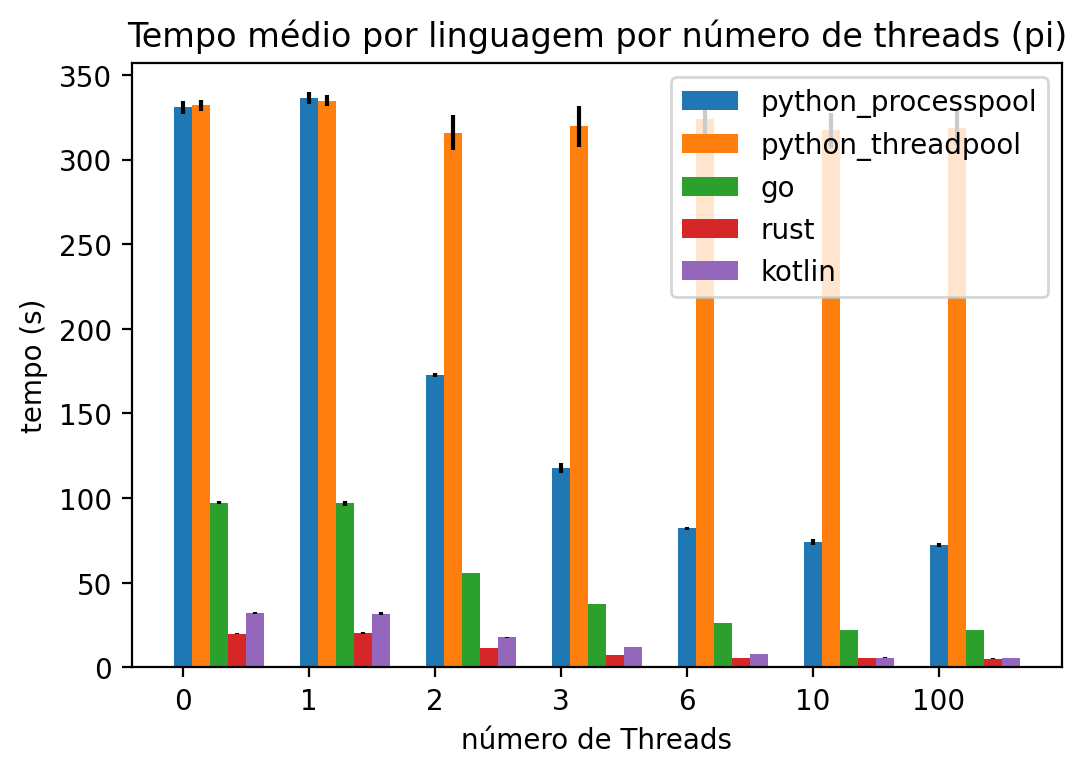
\includegraphics[width=1\textwidth]{tempo-medio-pi.png}
    \caption{tempo medio de computação do pi.}
    \label{fig:tempo medio pi}
\end{figure}

\begin{figure}[t] % t é pra ficar no topo
    \centering
    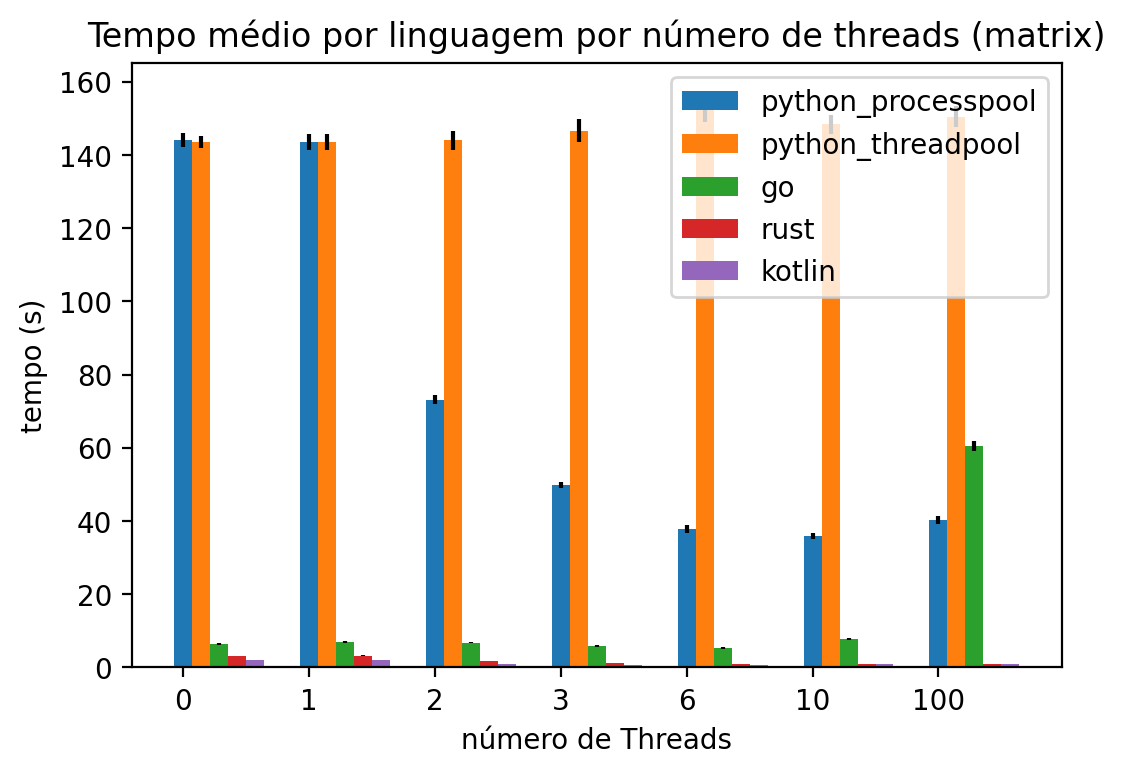
\includegraphics[width=1\textwidth]{tempo-medio-matrix.png}
    \caption{tempo medio de computação da matrix.}
    \label{fig:tempo medio matrix}
\end{figure}

Além de dificultar a visualização do efeito de paralelizar o código, o desempenho bruto das linguagens em cada uma das aplicações é de caráter secundário. Com isso em mente, os tempos de cada linguagem foram normalizados, tomando como parâmetro o tempo que cada uma levou na execução sequencial (0 threads). Produziu-se então os gráficos: \ref{fig:tempo medio norm pi} e \ref{fig:tempo medio norm matrix}

\begin{figure}[t] % t é pra ficar no topo
    \centering
    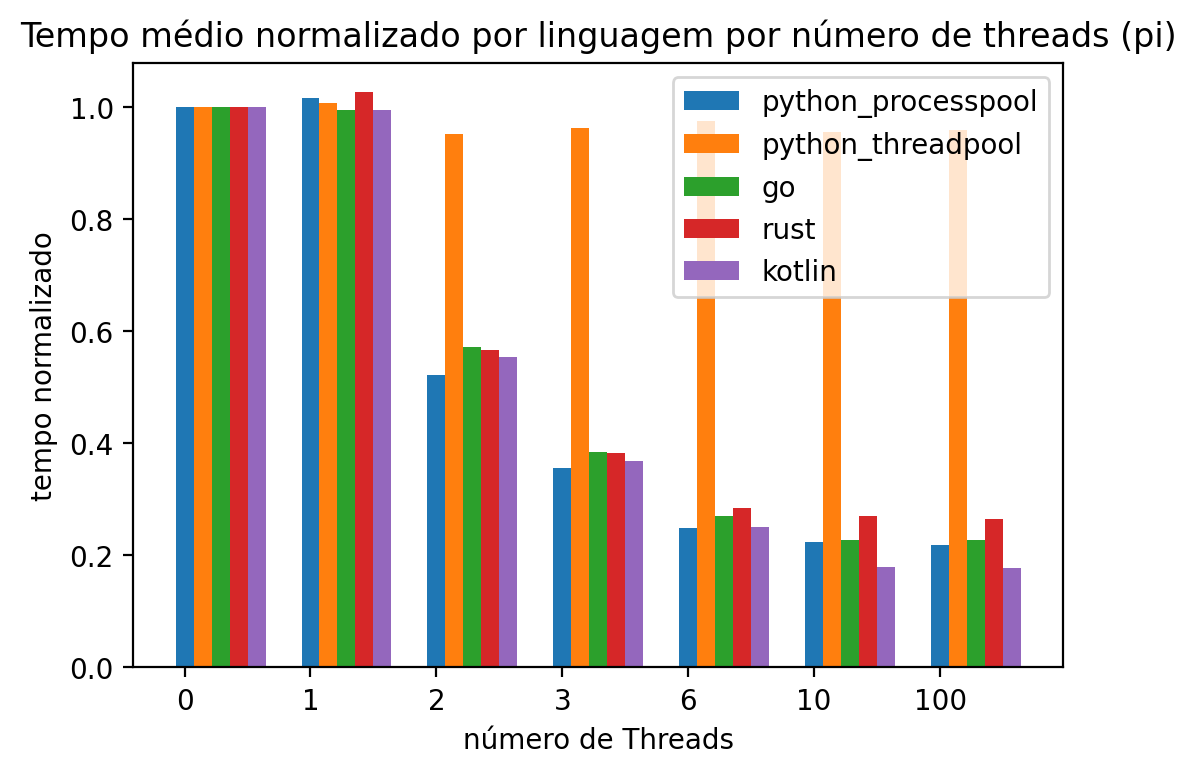
\includegraphics[width=1\textwidth]{tempo-medio-pi-normalizado.png}
    \caption{tempo medio normalizado de computação do pi.}
    \label{fig:tempo medio norm pi}
\end{figure}

\begin{figure}[t] % t é pra ficar no topo
    \centering
    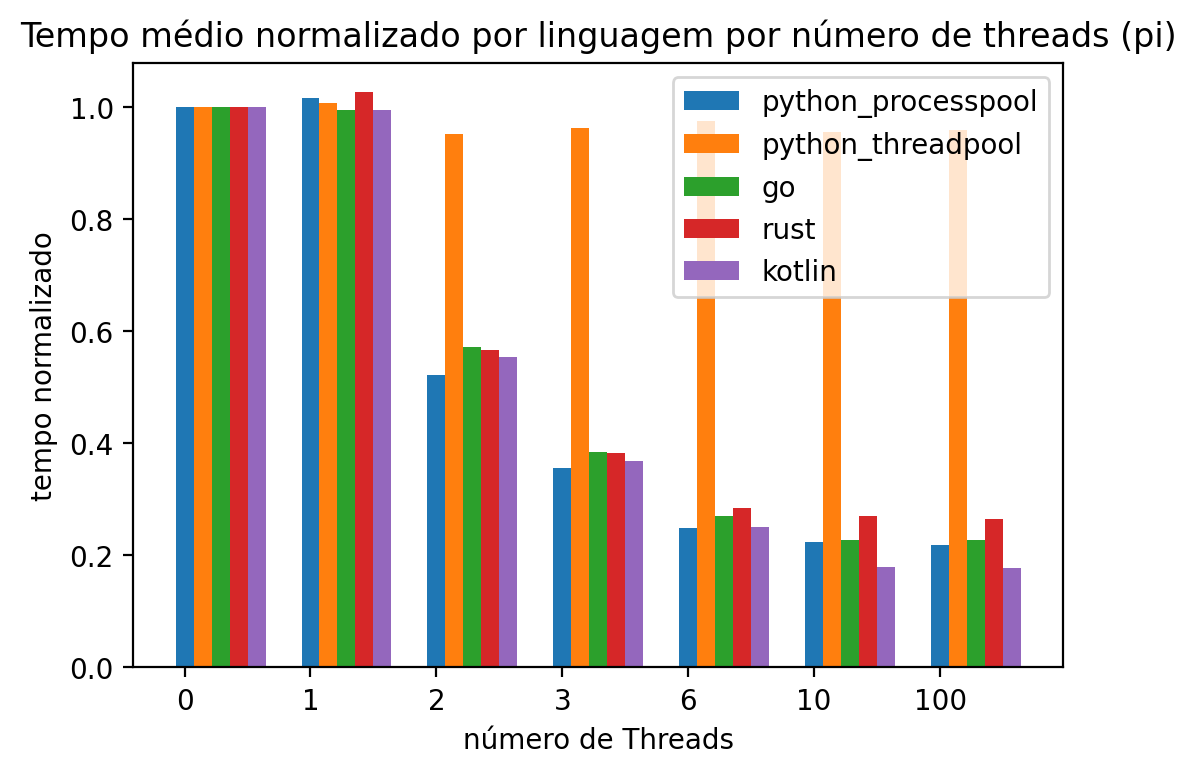
\includegraphics[width=1\textwidth]{tempo-medio-pi-normalizado.png}
    \caption{tempo medio normalizado de computação da matrix.}
    \label{fig:tempo medio norm matrix}
\end{figure}

Percebe-se também que o ganho de eficiência relativa de Rust não foi tão grande quanto de outras linguagens e supõe-se que isso se dê pelo fato de Rust utlizar threads de OS verdadeiras. É importante lembrar que os tempos absolutos de Rust foram melhores que a competição, e em tempos de execução mais curtos evidencia-se mais o custo de criação, gerenciamento e destruição de threads.

Go apresentou um desempenho muito satisfatório, tanto em tempo quanto em speedup. Contudo, Go mostrou-se incapaz de trabalhar apropriadamente com compartilhamento de memória, apresentando pouquíssimo speedup na multiplicação de matrizes.

% Por fim, acredita-se ser conveniente uma compilação final dos dados mostrando o \emph{speedup}, calculado como o inverso do tempo médio normalizado.

Esperava-se que, em python, \emph{process pooling} superasse \emph{thread pooling}, dado que não seriam usados algoritmos com nenhum IO. Na prática isso ocorreu. Mesmo assim, Python ficou atrás de todas as outras linguagens em eficiência bruta. Em termos de speedup, a linguagem se saiu bem, e acredita-se que seja pelo fato de o tempo gasto criando, destruindo e gerenciando as threads tenha sido diluído durante a longa execução. Vale reiterar que, de todas as linguagens, python é a única que não aceitava definições in-line de funções para serem enviadas para os criadores de threads, causando certo desconforto na hora de programar.

A expectativa de Rust superar (\emph{outperform}) as outras linguagens foi suprida. Percebe-se claramente sua superioridade sobre as outras em termos de velocidade, como esperado de uma linguagem de sistema, e a imensa disparidade de Python em relação às outras. Contudo, vale notar que ambos têm propósitos quase que diametralmente opostos: Python é de fácil adoção enquanto Rust foi uma das linguagens mais desafiadoras e trabalhosas.

Programar com Kotlin foi uma experiência frustrante pela influência da empresa JetBrains na documentação da linguagem e em seu ambiente, mas seu design é sólido e intuitivo. Fica claro que trata-se de uma linguagem voltada para o mercado, e com poderosas ferramentas de programação assíncronas, se presta bem ao desenvolvimento de aplicações para o sistema operacional Android. Seu desempenho na aplicação da multiplicação de matrizes foi particularmente surpreendente.

Inadvertidamente, a execução dos códigos de multiplicação de matrizes em 100 threads evidenciaram a memória consumida. Tratava-se de um teste prelimitar, pouco criterioso, no qual as aplicações dividiam a memória com outras aplicações, mas tanto Python quanto Go levaram muito mais do que esperado e supõe-se que seja fruto de exceder a memória disponível. As figuras \ref{fig:anomalia matrix GO} \ref{fig:anomalia matrix norm GO} evidenciam a falha no experimento com Go, mas não contribuem com dados relevantes para a comparação quantitativa. Vale ressaltar que este não era um objetivo primário do estudo, mas que a prática clareou as intuições do experimentador.


\begin{figure}[t] % t é pra ficar no topo
    \centering
    \includegraphics[width=1\textwidth]{anomalia-tempo-medio-matrix.png}
    \caption{anomalia em experimento preliminar com Go.}
    \label{fig:anomalia matrix GO}
\end{figure}

\begin{figure}[t] % t é pra ficar no topo
    \centering
    \includegraphics[width=1\textwidth]{anomalia-tempo-medio-matrix-norm.png}
    \caption{anomalia em experimento preliminar com Go, tempos normalizados.}
    \label{fig:anomalia matrix norm GO}
\end{figure}


\newpage
%-------------------------------
% CONCLUSÃO
%-------------------------------
\section{Conclusão}
\label{sec:conclusao}

O prospecto para programação paralela e concorrente é bastante promissor. As linguagens estudadas se mostraram muito competentes dentro de seus nichos e disponibilizam diversos métodos clássicos de paralelismo e ferramentas consagradas de travas e sincronização. Além disso, cada uma, em seu modo, inovou, melhorando ergonomia e segurança, incorporando em seu projeto garantias e conceitos fascinantes como borrow checker de Rust ou corrotinas em Go e Kotlin.
De todas as linguagens a mais decepcionante foi Python, que apesar de acessível, foi superada por Go quando se trata de concorrência e paralelismo, além de ficar muito atrás em termos de eficiência. Seu lugar continua garantido como uma linguaegm popular, contudo, por seu riquíssimo ecossistema e comunidade engajada e diversa.

Com \emph{breakthroughs} tecnológicos cada vez mais difíceis no mundo dos transistores e a Lei de Moore em risco, acredita-se que a acessibilidade de paralelismo e concorrência em linguagens \emph{mainstream} se torne uma prioridade cada vez mais alta.




\newpage
%-------------------------------
% BIBLIOGRAFIA
%-------------------------------
\singlespacing

\bibliographystyle{apalike}
\bibliography{refs.bib}

\end{document}
